\documentclass{article}
\usepackage{amsmath}
\usepackage{siunitx}
\usepackage{xcolor}
\usepackage{hyperref}
\usepackage{graphicx}
\usepackage{listings}
\lstset{language=Python,%
	basicstyle=\footnotesize\ttfamily,stringstyle=\color{red!40!black},%
	commentstyle=\color{violet!95!black}\textsf,%
	keywordstyle=\color{green!30!black}, morekeywords={as},%
	tabsize=3,breaklines=true,postbreak=\mbox{\textcolor{red}{$\hookrightarrow$}\space}, showstringspaces=false,%
	backgroundcolor = \color{black!3!white}}
\usepackage[a4paper, left=2cm, right=2cm, top=2cm, bottom=2cm]{geometry}

\newcommand{\nota}[1]{\textcolor{red}{#1}}
\newcommand{\arbitrario}[1]{\textcolor{blue}{#1}}

\author{Marco Codato}
\title{Notes}

\begin{document}
\maketitle

\section{Introduction}

Moved to the GitHub repository  \href{https://github.com/codatomrc/tesi}{\texttt{codatomrc/tesi}}.

\section{Background spectrum extraction}

\subsection{Automatic detection}
The script I am writing works as follows.
\begin{itemize}
	\item Automatically explores a directory and find all the raw files, marked as \texttt{filename.fc.fits}. All the files are then processed one by one.
	
	\item Far each frame relevant information is extracted from the header (hdr). In particular the script requires
	\begin{itemize}
		\item information about the wavelength of each pixel (initial wavelength, increment of each pixel and width of the detector and horizontal binning factor),
		\item slit width and length (thus the detector height an vertical binning factor, aside the CCD scale),
		\item year of observation
	\end{itemize}
	\item For each frame a preliminary integration over all the wavelenghts is performed by summing the data in the file along the dispersion direction. This is an efficient way of detecting astronomical sources, that are spatially limited, against the background, supposed uniform along the slit.
	
	\item \arbitrario{I preliminarly decided to cut blue wavelengths at \SI{3500}{\angstrom}. This value was bull-eyed looking at bkg spectra and relizing that this is the treshold where the noise becomes dominant.}
	
	\item Cosmic rays and excessive noise are removed. In particular in the bluer part of the spectrum, due to the low sensitivity of the detector, after the flux calibration the noise is extremely high, seriously affecting the quality of the measurements. For example see the image below
	\begin{figure}[h!]
		\centering
		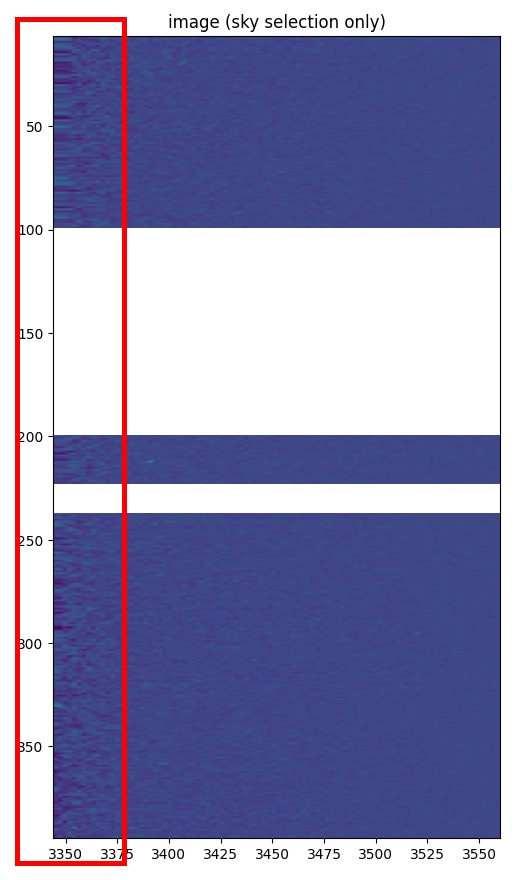
\includegraphics[width=.35\textwidth, angle=90]{10_det}
	\end{figure}
	I removed these features by scanning each column of the frame looking for bright sharp peaks. \arbitrario{Some good settings to remove both cosmic rays and noise is to find peaks very thin, with a width less than 3\,px and an height of more than 5 times the average level of the bkg} (i.e.\ the value estimated from the luminosity profile, divided by the number of pixels along the horizontal direction) \textcolor{red}{bisognerebbe stimare la dimensione apparente dei raggi cosmici e confrontarla con la scala sul CCD per essere sicuri che funzioni con tutte le immagini}.
	
	The peaks were identified with the function \href{https://docs.scipy.org/doc/scipy/reference/generated/scipy.signal.find_peaks.html}{\texttt{scipy.signal.find\_peaks}} while their FWHM was estimated with \href{https://docs.scipy.org/doc/scipy/reference/generated/scipy.signal.peak_widths.html#scipy.signal.peak_widths}{\texttt{scipy.signal.peak\_widths}}. To be sure all the cosmic ray trace or the noise fluctuation was contained in the detected width I added a further 1\,px on both directions along the columns.
	
	\item \arbitrario{The columns that afeter the cleaning are depleted of more than the 25\% their pixels are discarted as they are very likely to be noisy columns.}
	
	\item On the cleaned frame I take again luminosity profile along the slit (i.e.\ integration on the wavelengths) to search for the astronomical sources.
	Some of the frames present a systematic trend in the bkg which makes the source detection not trivial. I decided to proceed as follows:
	\begin{enumerate}
		\item Estimate the general trend of the luminosity profile. \arbitrario{I used a biweighted detrending algorithm with a windowing of 200\,px and the fine-tuning parameter \texttt{cval=10}}, using the function \href{https://github.com/hippke/wotan}{\texttt{wotam.flatten}}. Such large window size is still not enough to cancel out the effect of the brightest features.
		\item \arbitrario{Trim the original light profile} by removing all the data that emerges from the bkg global trend. \arbitrario{I uesd as treshold the detrended profile, vertically shifted by a factor equal to the 5\% of the average bkg level}. A good estimator for the avg bkg level turned to be the median of the original light profile.
		\item \arbitrario{Perform a new detrend on the trimmed data}. In this case I used a much narrower windows size, \arbitrario{or 50\,px} since it was not necessary to dilute the bright peaks in correspondence of the sources. This can be considered as an estimator for the global bkg trend along the slit.
	\end{enumerate}
	\begin{figure}[h!]
		\centering
		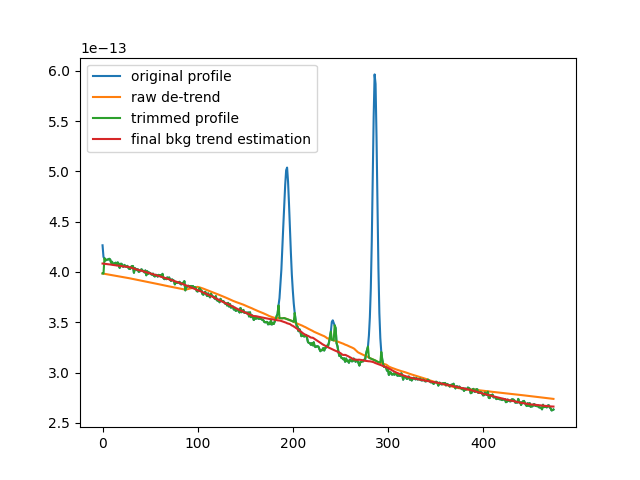
\includegraphics[width=.65\textwidth]{detrend_example}
	\end{figure}
	\item The source peaks are detected automatically with \texttt{scipy.signal.find\_peaks}. Peaks were identified after removing the contribution of the systematic bkg trend detected in the previous step. \arbitrario{I selected only those features with a width larger than 3\,px (to be sure not to include unremoved cosmic rays) and an height greater than the 5\% of the bkg (median) level.}
	
	\item I computed the width of the sources with \texttt{scipy.signal.peak\_widths}. \arbitrario{In particular I considered the FWHM which proved to be more solid than the total width. Since many kinds of astronomical sources have a central core and bright wings, I decided to remove a that span $2.5\times\text{FWHM}$ wrt the center of the peak to take into account such wings.}	
	In some cases the luminosity profile of the sources is not gaussian and the tails are brighter than the gaussian prevision. In these cases I considered as related to a source also all the pixels arounf the peak that are brighter than what expected from the detrended profile.
	
	\item At the end the script produces:
	\begin{itemize}
		\item A plot of the luminosity profile along the slit (the one from the original frame, and after the cosmic ray removal) plus the masked source regions.
		\item The bkg spectrum from the selected rows only, integrated along the spatial direction (plus the same for the full cleaned frame as a comparison).
		\item A new file where cosmic rays, the UV noise and the astronomical sources are removed. The information in the hdr are preserved and the data when the file was produced is added.
	\end{itemize}
\end{itemize}


\paragraph{A quantitative approach.} I tried to sketch a qualitative model where I assumed gaussian profiles of the sources. The source ended when its flux was comparable to the amplitude of the bkg noise. The final distance $\Delta$ from the center of the source was
\[\Delta = \frac{1}{2\sqrt{2\ln 2}}\text{FWHM}\sqrt{\ln(S_\text{max}^2/B)}   \]
where $S_\text{max}$ was the maximum counts of the source, while $B$ the average level of bkg around the object. Since many extended objects cannot be reproduced by gaussian profiles this estimation may be misleading in many cases. Since the empirical procedure discussed above seems quite solid with current data, implementing a rigorous analytical approach that accounts for different luminosity profiles of the sources, is definitively unecessary.


\subsection{Comments on the first results}

\paragraph{Frame limitations(?)} I wonder whether the whole CCD area is suitable for collecting data or it would be better/necessary to neglect some specific regions, both in the spatial and dispersion directions.

\textcolor{red}{What about the lines ``\texttt{CCDSEC}'' and ``\texttt{BIASSEC}'' in the header of the frames?}


\section{Bkg analysis}
Once the bkg is extraced from each frame and saved into a new one, I can develope a script that reads the new filtered files and process them automatically.

\subsection{Line analysis}
I want to measure most of the spectral lines containted in sky spectra and reported in the table \texttt{tesi/lines.txt}. I particular I am interested in the equivalent width (EW). Eventually I also shall try to indentify further lines, e.g.\ the bright one at $\sim\SI{3800}{\angstrom}$. The procedure I plan to follow is the following
\begin{itemize}
	\item Average all the px in each column in the original 2D frame to get the bkg unidimensional spectrum.
	\item Identify the positions of the known lines (table \texttt{lines.txt}) in the spectra. Note that due to the low resolution of the frames, some lines are totally unresolved. \arbitrario{I will consider as single unresolved lines, those with a wavelength difference lower than 1 time the pixel resolution} (which is of the order of $\sim\SI{3}{\angstrom}$).
	\item Once identified the lines I want to fit them with some Gaussian profiles to estimate their width and thus compute the EW analitically from the best fit profile. The regions and the number of lines are choosen \textit{a priori} and are the same for all the spectra. I selected the boundaries of the fitting regions to avoid other minor lines or features that could be bias the measurements of the line or the continuum. In the table \texttt{tesi/ranges} is contained such information.
	\item I can fit some limited areas of the spectra around the lines, and fit each of these areas with some gaussians profiles for the lines plus a polynomial (probably just linear profile) for the underlying continuum.
\end{itemize}

\subsection{Tentative analysis on the whole spectra}

\paragraph{Date correlation.}
Bkg spectra are chacarterized by few very bright emission lines plus one/two continuum region(s). A very first analisys may consist on lower the resolution of the spectra and compare them with each others. \arbitrario{In particular I decided to bin them in \SI{100}{\angstrom} bin size and crhonologically order them.}
\begin{figure}[h!]
	\centering
	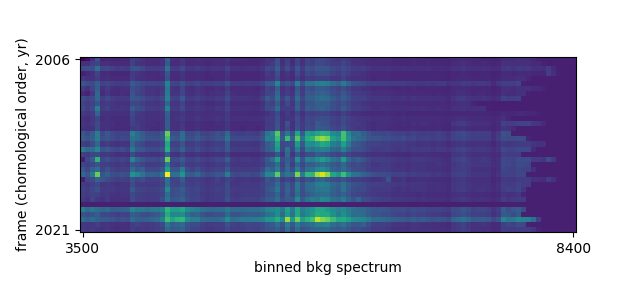
\includegraphics[width=.75\textwidth]{../Figure_1}
\end{figure}
Data seems to be consistent with the claim that the bkg level has increased in the years, likely due to artifical light.

\paragraph{Orientation correlation.} I plotted the position of each frame on the sky sphere (in terms of airmass and azimuth) against the total luminosity of each spectrum (i.e.\ integrated in the wavelengths).
\begin{figure}[h!]
	\centering
	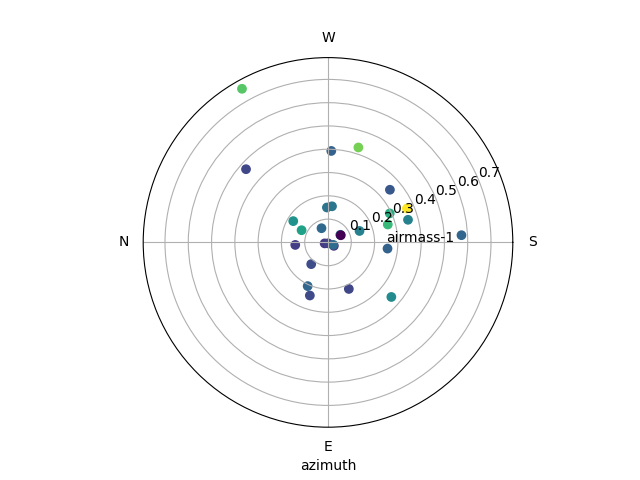
\includegraphics[width=.75\textwidth]{../radial}
\end{figure}
Appartently brightest measurements are concentrated towar the S/W direction.

\paragraph{Moon and Sun position correlations.}
I checked whether the position of Moon and Sun affected the total bkg counts. The quantities I checked against the total flux are the Sun altitude below the horizon, the angular separation of from the moon and the moon phase at the epoch of observation.
	\begin{figure}[h!]
	\centering
	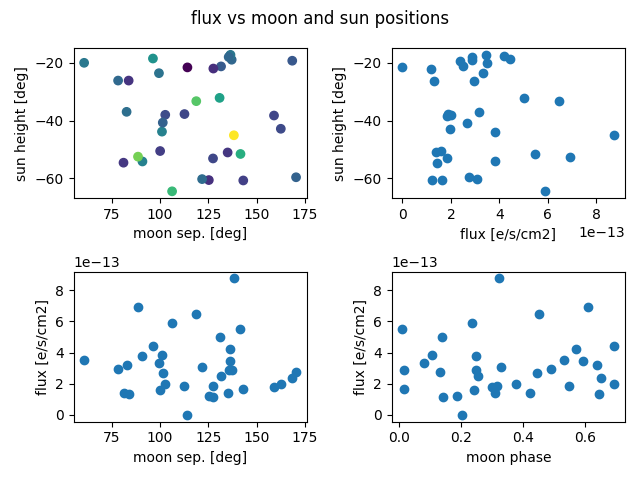
\includegraphics[width=.75\textwidth]{../positions}
\end{figure}
No evident trends emerged from this analysis, althought this is to the smartest choiche for the plotted quantities. For example all of the 3 quantities of the plot must be considered at the same time since their effects should sum up.

\paragraph{Spectral features correlation.} I checked for correlations in the binned spectra by computing the covariance matrix of binned data. I normalized the spectra with their value on the 58-th bin, i.e.\ at $\sim\SI{6450}{\angstrom}$, a region of the bkg spectrum where no relevant continuum nor evident lines are present.  Resulting correlations have to be further investigated.
	\begin{figure}[h!]
	\centering
	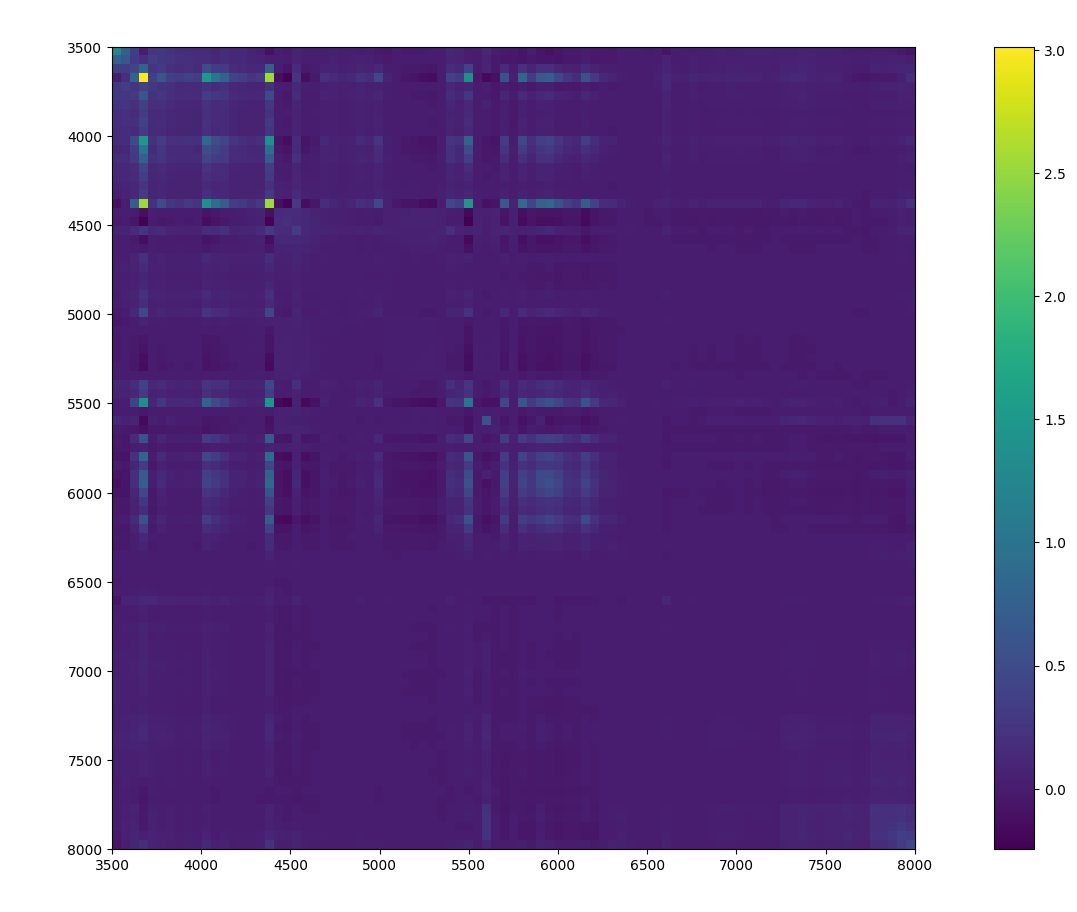
\includegraphics[width=.75\textwidth]{../covariance}
\end{figure}

\newpage
\section{Appendix: Python codes}
\subsection{Bkg extraction code}
\lstinputlisting[language=Python]{../bkg_extractor.py}
\subsection{Bkg analysis code}
\lstinputlisting[language=Python]{../bkg_analyzer.py}

\end{document}

